\documentclass[table]{beamer}
\mode<presentation>
\usetheme{Berlin}
\usecolortheme{beaver}
\usepackage{listings}
\usepackage{multirow}
\usepackage{xcolor}

%%%
% LISTINGS SETTING
\lstset{ %
  backgroundcolor=\color{yellow},   % choose the background color; you must add \usepackage{color} or \usepackage{xcolor}
  basicstyle=\tiny\ttfamily,        % the size of the fonts that are used for the code
  breakatwhitespace=false,         % sets if automatic breaks should only happen at whitespace
  breaklines=true,                 % sets automatic line breaking
  captionpos=b,                    % sets the caption-position to bottom
  commentstyle=\color{red},    % comment style
  deletekeywords={...},            % if you want to delete keywords from the given language
  escapeinside={\%*}{*)},          % if you want to add LaTeX within your code
  extendedchars=true,              % lets you use non-ASCII characters; for 8-bits encodings only, does not work with UTF-8
  frame=single,                    % adds a frame around the code
  keepspaces=true,                 % keeps spaces in text, useful for keeping indentation of code (possibly needs columns=flexible)
  keywordstyle=\color{blue},       % keyword style
%  language=Octave,                 % the language of the code
  morekeywords={*,...},            % if you want to add more keywords to the set
  numbers=left,                    % where to put the line-numbers; possible values are (none, left, right)
  numbersep=5pt,                   % how far the line-numbers are from the code
  numberstyle=\tiny\color{gray}, % the style that is used for the line-numbers
  rulecolor=\color{black},         % if not set, the frame-color may be changed on line-breaks within not-black text (e.g. comments (green here))
  showspaces=false,                % show spaces everywhere adding particular underscores; it overrides 'showstringspaces'
  showstringspaces=false,          % underline spaces within strings only
  showtabs=false,                  % show tabs within strings adding particular underscores
  stepnumber=1,                    % the step between two line-numbers. If it's 1, each line will be numbered
  stringstyle=\color{mauve},     % string literal style
  tabsize=4,                       % sets default tabsize to 2 spaces
  title=\lstname                   % show the filename of files included with \lstinputlisting; also try caption instead of title
}


%%%
% TITLE PREAMBLE
\title[Intro to Bioinformatics] % (optional, only for long titles)
{An Introduction to Bioinformatics Tools}
\subtitle{Part 3: Workshop}
\author[Pritchard, Cock] % (optional, for multiple authors)
{Leighton~Pritchard \and Peter~Cock}
\institute[The James Hutton Institute] % (optional)
{
  Information and Computational Sciences\\
  The James Hutton Institute
}
\date[May 2014] % (optional)
{Bioinformatics Training, 29$^{th}$,30$^{th}$ May 2014}
\subject{Bioinformatics}

%%%
% TOC
% Show table of contents, with current section highlighted,
% at the start of each section
\AtBeginSection[]
{
  \begin{frame}
    \frametitle{Table of Contents}
    \tableofcontents[currentsection,hideothersubsections]
  \end{frame}
}


%%%
% START DOCUMENT
\begin{document}

  \frame[plain]{\titlepage}
  
%%%
% SECTION: Workshop Outline
  \section{Outline}
 
    % What you will be doing
    \begin{frame}
     \frametitle{What You Will Be Doing}
     \begin{itemize}
       \item Functional annotation of a draft bacterial genome
       \begin{itemize}
         \item Genome comparisons
         \item Gene prediction/ORF detection
         \item Gene functional annotation
         \item Gene comparisons
       \end{itemize}
     \end{itemize}
    \end{frame}
    
    \begin{frame}
     \frametitle{Genome comparisons}
     \begin{itemize}
       \item Artemis
       \item BLAST
       \item MUMmer
       \item MAUVE
       \item ACT
       \item Differences between genome aligners
     \end{itemize}
    \end{frame}

    \begin{frame}
     \frametitle{Gene (coding sequence) Prediction}
     \begin{itemize}
       \item ORF detection
       \item GeneMark
       \item Glimmer
       \item Prodigal
       \item Benchmarking gene prediction
     \end{itemize}
    \end{frame}

    \begin{frame}
     \frametitle{Functional Prediction}
     \begin{itemize}
       \item InterPro
       \item RAST
       \item KAAS
       \item PFam
       \item Artemis
       \item Functional classification
     \end{itemize}
    \end{frame}
    
    \begin{frame}
     \frametitle{Gene Comparisons}
     \begin{itemize}
       \item BLAST
       \item HMMer
       \item CLUSTAL
       \item T-COFFEE
       \item JalView
       \item Differences between gene aligners
     \end{itemize}
    \end{frame}


  % Getting started
  \section{Load Sequence Data}
  \begin{frame}
    \frametitle{Locate your data}
    \begin{itemize}
      \item You are in group A, B, C or D - this decides your chromosome sequence: \\
      \texttt{chrA.fasta}, \texttt{chrB.fasta}, \texttt{chrC.fasta}, \texttt{chrD.fasta}
      \item Each sequence represents a single stitched, ordered draft bacterial genome comprising a number of contigs.
      \item You will use your sequence as the basis of the exercises in the workshop.
    \end{itemize}
  \end{frame}  
  
  \begin{frame}
    \frametitle{Locate your data}
    \begin{itemize}
      \item You are in group A, B, C or D - this decides your dataset: \\
      \texttt{chrA.fasta}, \texttt{chrB.fasta}, \texttt{chrC.fasta}, \texttt{chrD.fasta}
      \item You also have a GFF file describing the location of assembled contigs \\
      \texttt{chrA\_contigs.gff}, \texttt{chrB\_contigs.gff}, \texttt{chrC\_contigs.gff}, \texttt{chrD\_contigs.gff}
      \item Your data is in \texttt{data/workshop/chromosomes}
    \end{itemize}
  \end{frame}    
  
% [fragile] frames must end with \end{frame} directly following a newline, or they break!
  \begin{frame}[fragile]
    \frametitle{Inspect the data}
    \begin{lstlisting}[language=bash]
$ cd ../../data/workshop/chromosomes
$ head -n 3 chrA.fasta 
>chrA
ttttcttgattgaccttgttcgagtggagtccgccgtgtcactttcgctttggcagcagt
gtcttgcccgtttgcaggatgagttacctgccacagaattcagtatgtggatacgcccgt
$ head -n 3 chrA_contigs.gff 
##gff-version 3
chrA	stitching	contig	1	154993	.	.	.	ID=contig00005_b;Name=contig00005_b
chrA	stitching	contig	155036	241491	.	.	.	ID=contig00018;Name=contig00018
    \end{lstlisting}
\end{frame}  

% [fragile] frames must end with \end{frame} directly following a newline, or they break!
  \begin{frame}[fragile]
    \frametitle{Download a Comparator Sequence}
    You will use \texttt{wget}, a powerful command-line tool for downloading data from the web
    \begin{lstlisting}[language=bash]
$ wget ftp://ftp.ncbi.nih.gov/genomes/Bacteria/Pectobacterium_atrosepticum_SCRI1043_uid57957/NC_004547.ffn
--2014-05-20 19:11:24--  ftp://ftp.ncbi.nih.gov/genomes/Bacteria/Pectobacterium_atrosepticum_SCRI1043_uid57957/NC_004547.ffn
           => 'NC_004547.ffn'
Resolving ftp.ncbi.nih.gov... 130.14.250.7, 2607:f220:41e:250::12
Connecting to ftp.ncbi.nih.gov|130.14.250.7|:21... connected.
Logging in as anonymous ... Logged in!
==> SYST ... done.    ==> PWD ... done.
==> TYPE I ... done.  ==> CWD (1) /genomes/Bacteria/Pectobacterium_atrosepticum_SCRI1043_uid57957 ... done.
==> SIZE NC_004547.ffn ... 4913065
==> PASV ... done.    ==> RETR NC_004547.ffn ... done.
Length: 4913065 (4.7M) (unauthoritative)

100%[====================>] 4,913,065    118KB/s   in 79s    

2014-05-20 19:12:46 (60.9 KB/s) - 'NC_004547.ffn' saved [4913065]
$ ls NC*
NC_004547.ffn
    \end{lstlisting}
\end{frame}  


  % Artemis
  \subsection{Artemis}
% [fragile] frames must end with \end{frame} directly following a newline, or they break!
  \begin{frame}[fragile]
    \frametitle{Inspect the data}
    Starting \texttt{Artemis}
    \begin{lstlisting}[language=bash]
$ art &
    \end{lstlisting}
    \begin{center}
      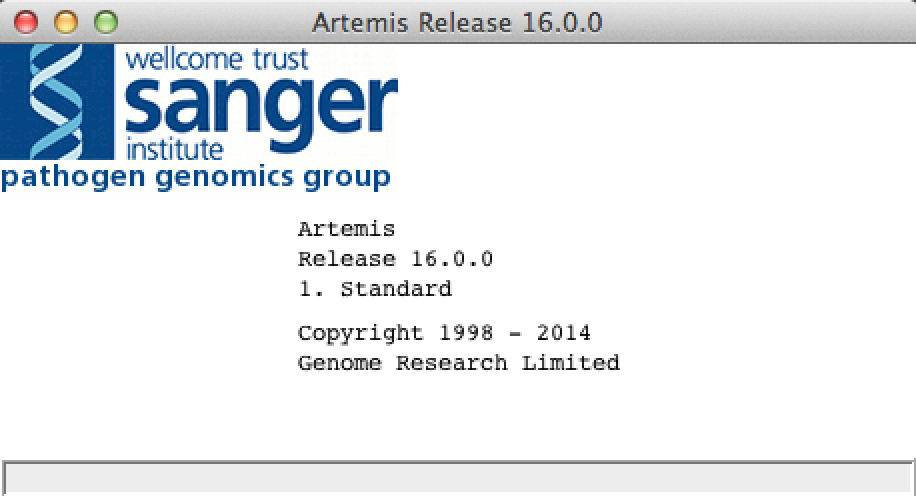
\includegraphics[width=0.6\textwidth]{images/artemis_splash} 
    \end{center}
\end{frame} 
    
  \begin{frame}
    \frametitle{Load the chromosome sequence}
    \begin{center}
      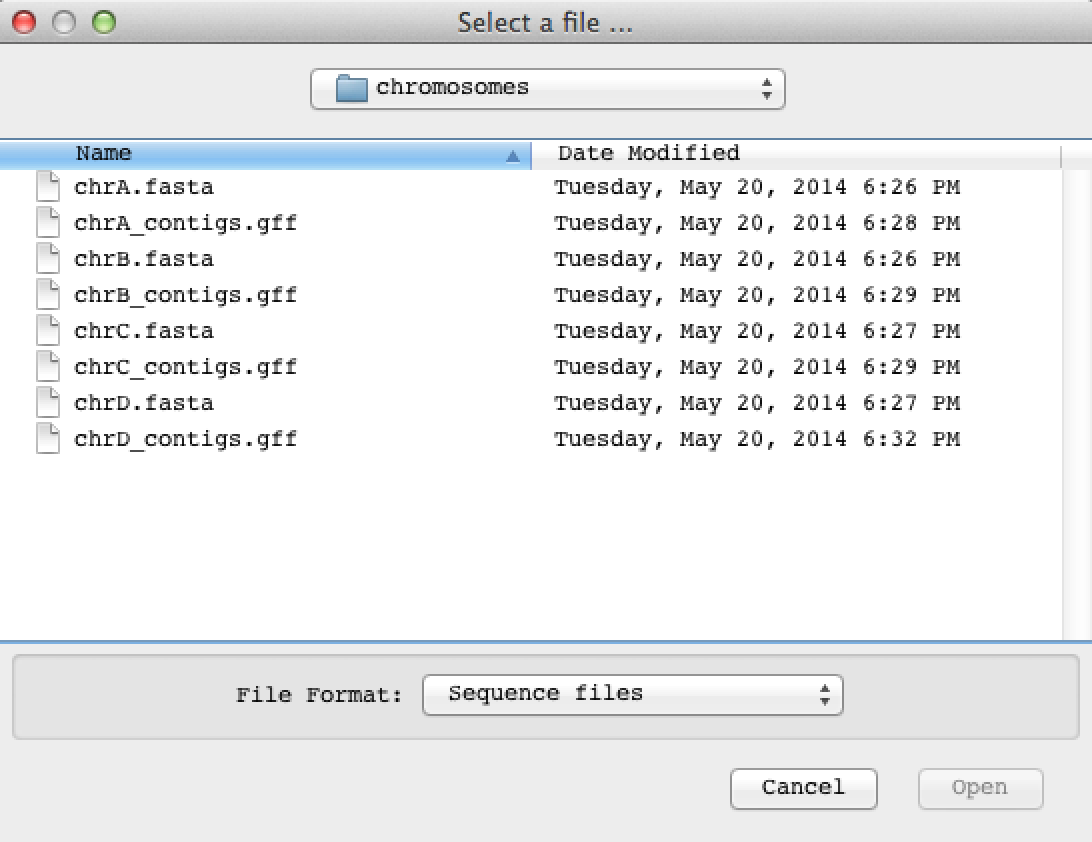
\includegraphics[width=0.75\textwidth]{images/artemis_files} 
    \end{center}
\end{frame}     
    
  \begin{frame}
    \frametitle{Load the chromosome sequence}
    \begin{center}
      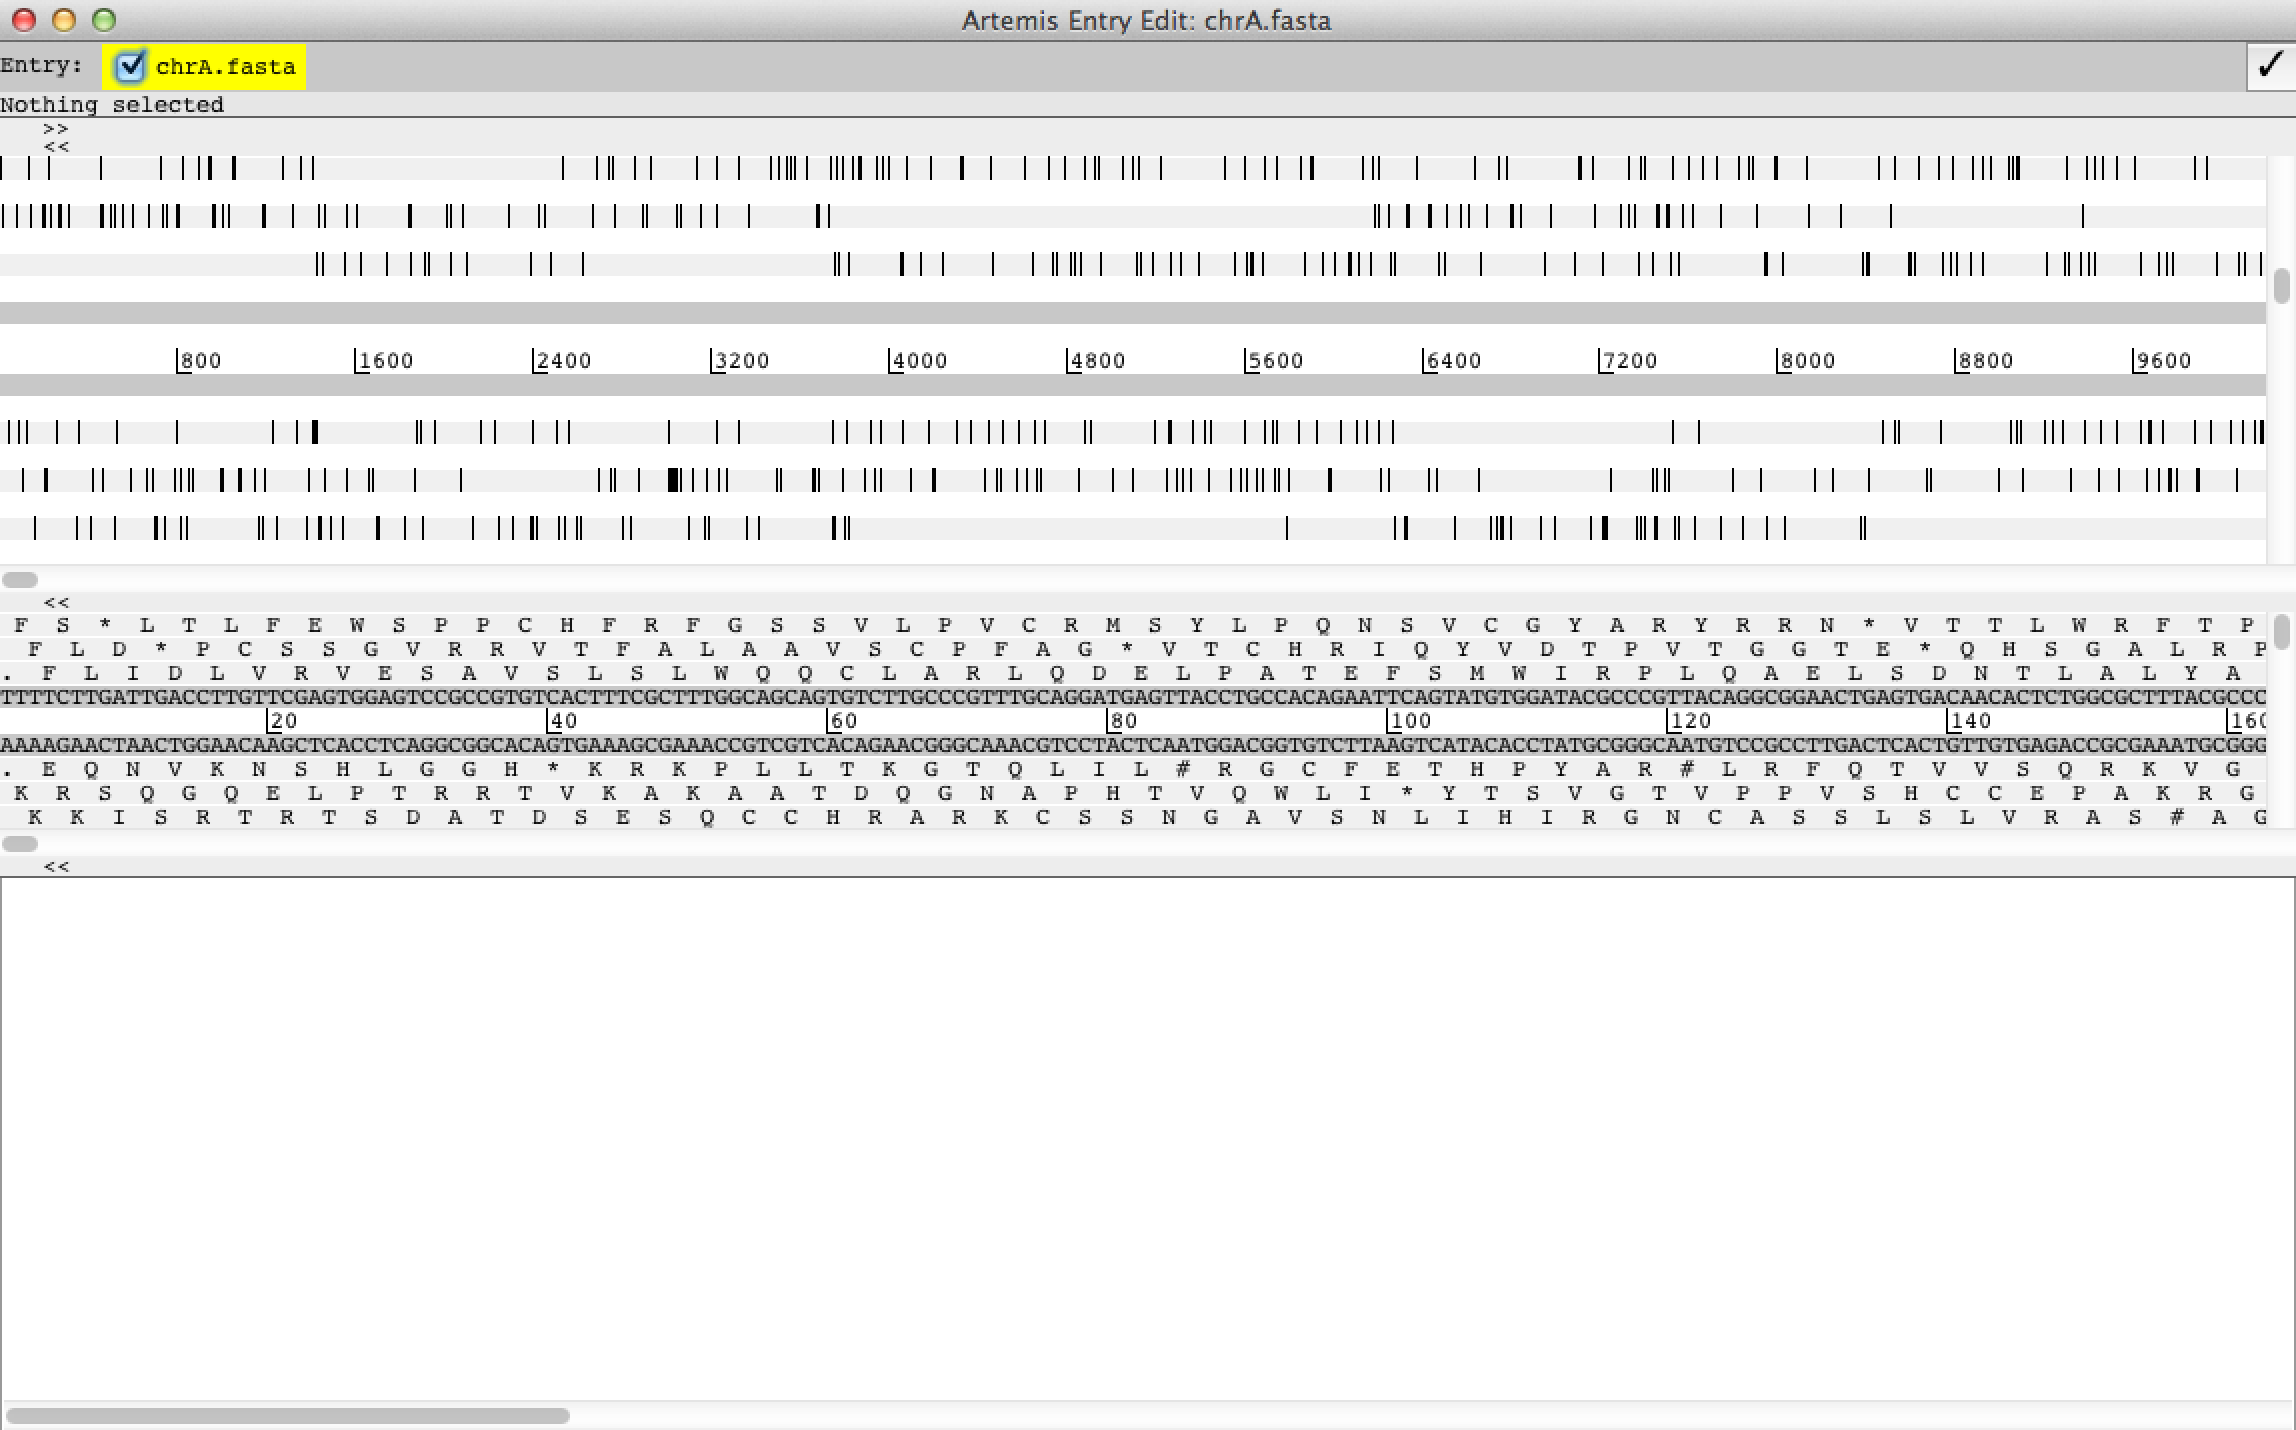
\includegraphics[width=0.8\textwidth]{images/artemis_loaded_seq} 
    \end{center}
\end{frame}     

  \begin{frame}
    \frametitle{Load the contig GFF}
    \begin{center}
      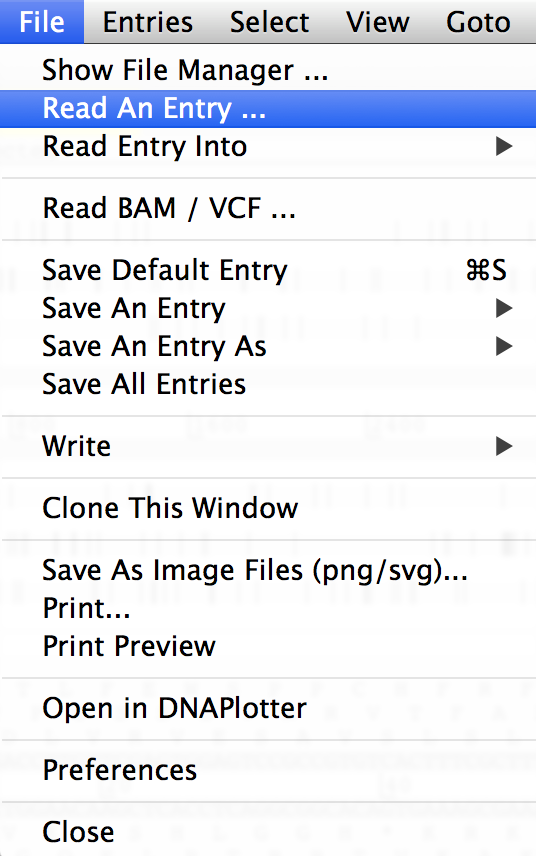
\includegraphics[width=0.3\textwidth]{images/artemis_read_entry} 
    \end{center}
\end{frame}     

  \begin{frame}
    \frametitle{Load the contig GFF}
    \begin{center}
      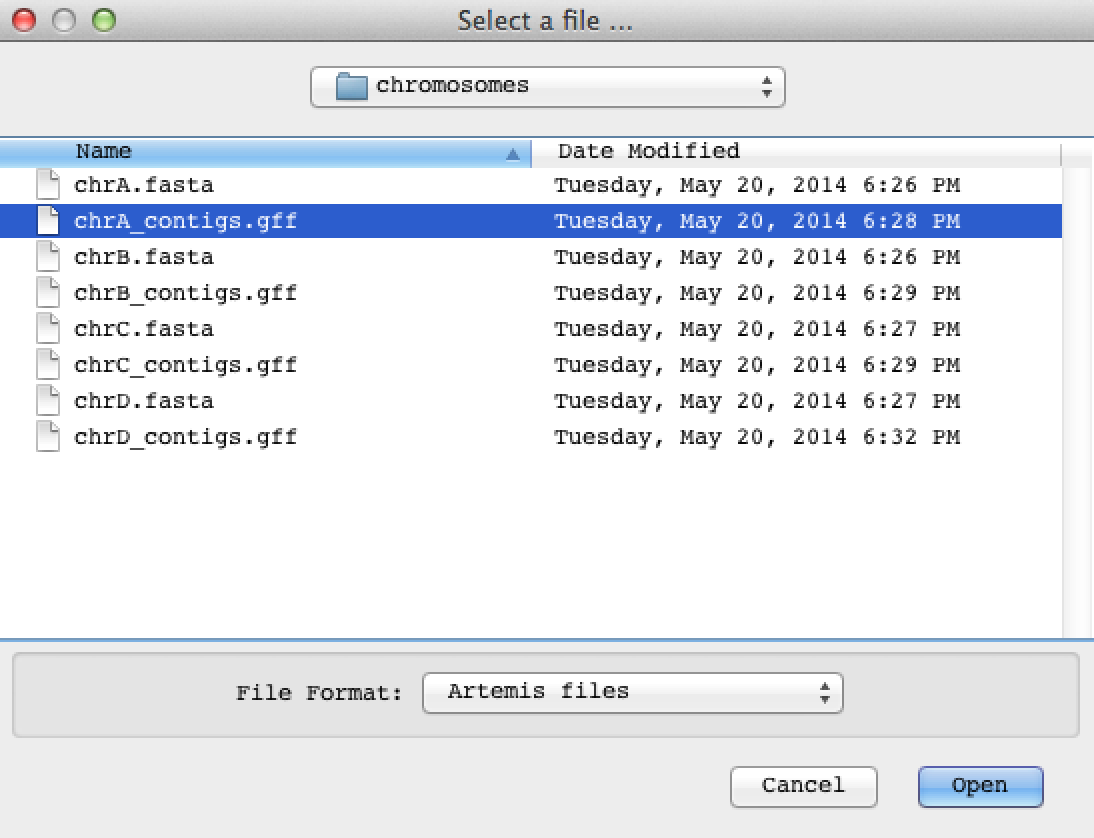
\includegraphics[width=0.75\textwidth]{images/artemis_select_contig_gff} 
    \end{center}
\end{frame}     

  \begin{frame}
    \frametitle{Load the contig GFF}
    \begin{center}
      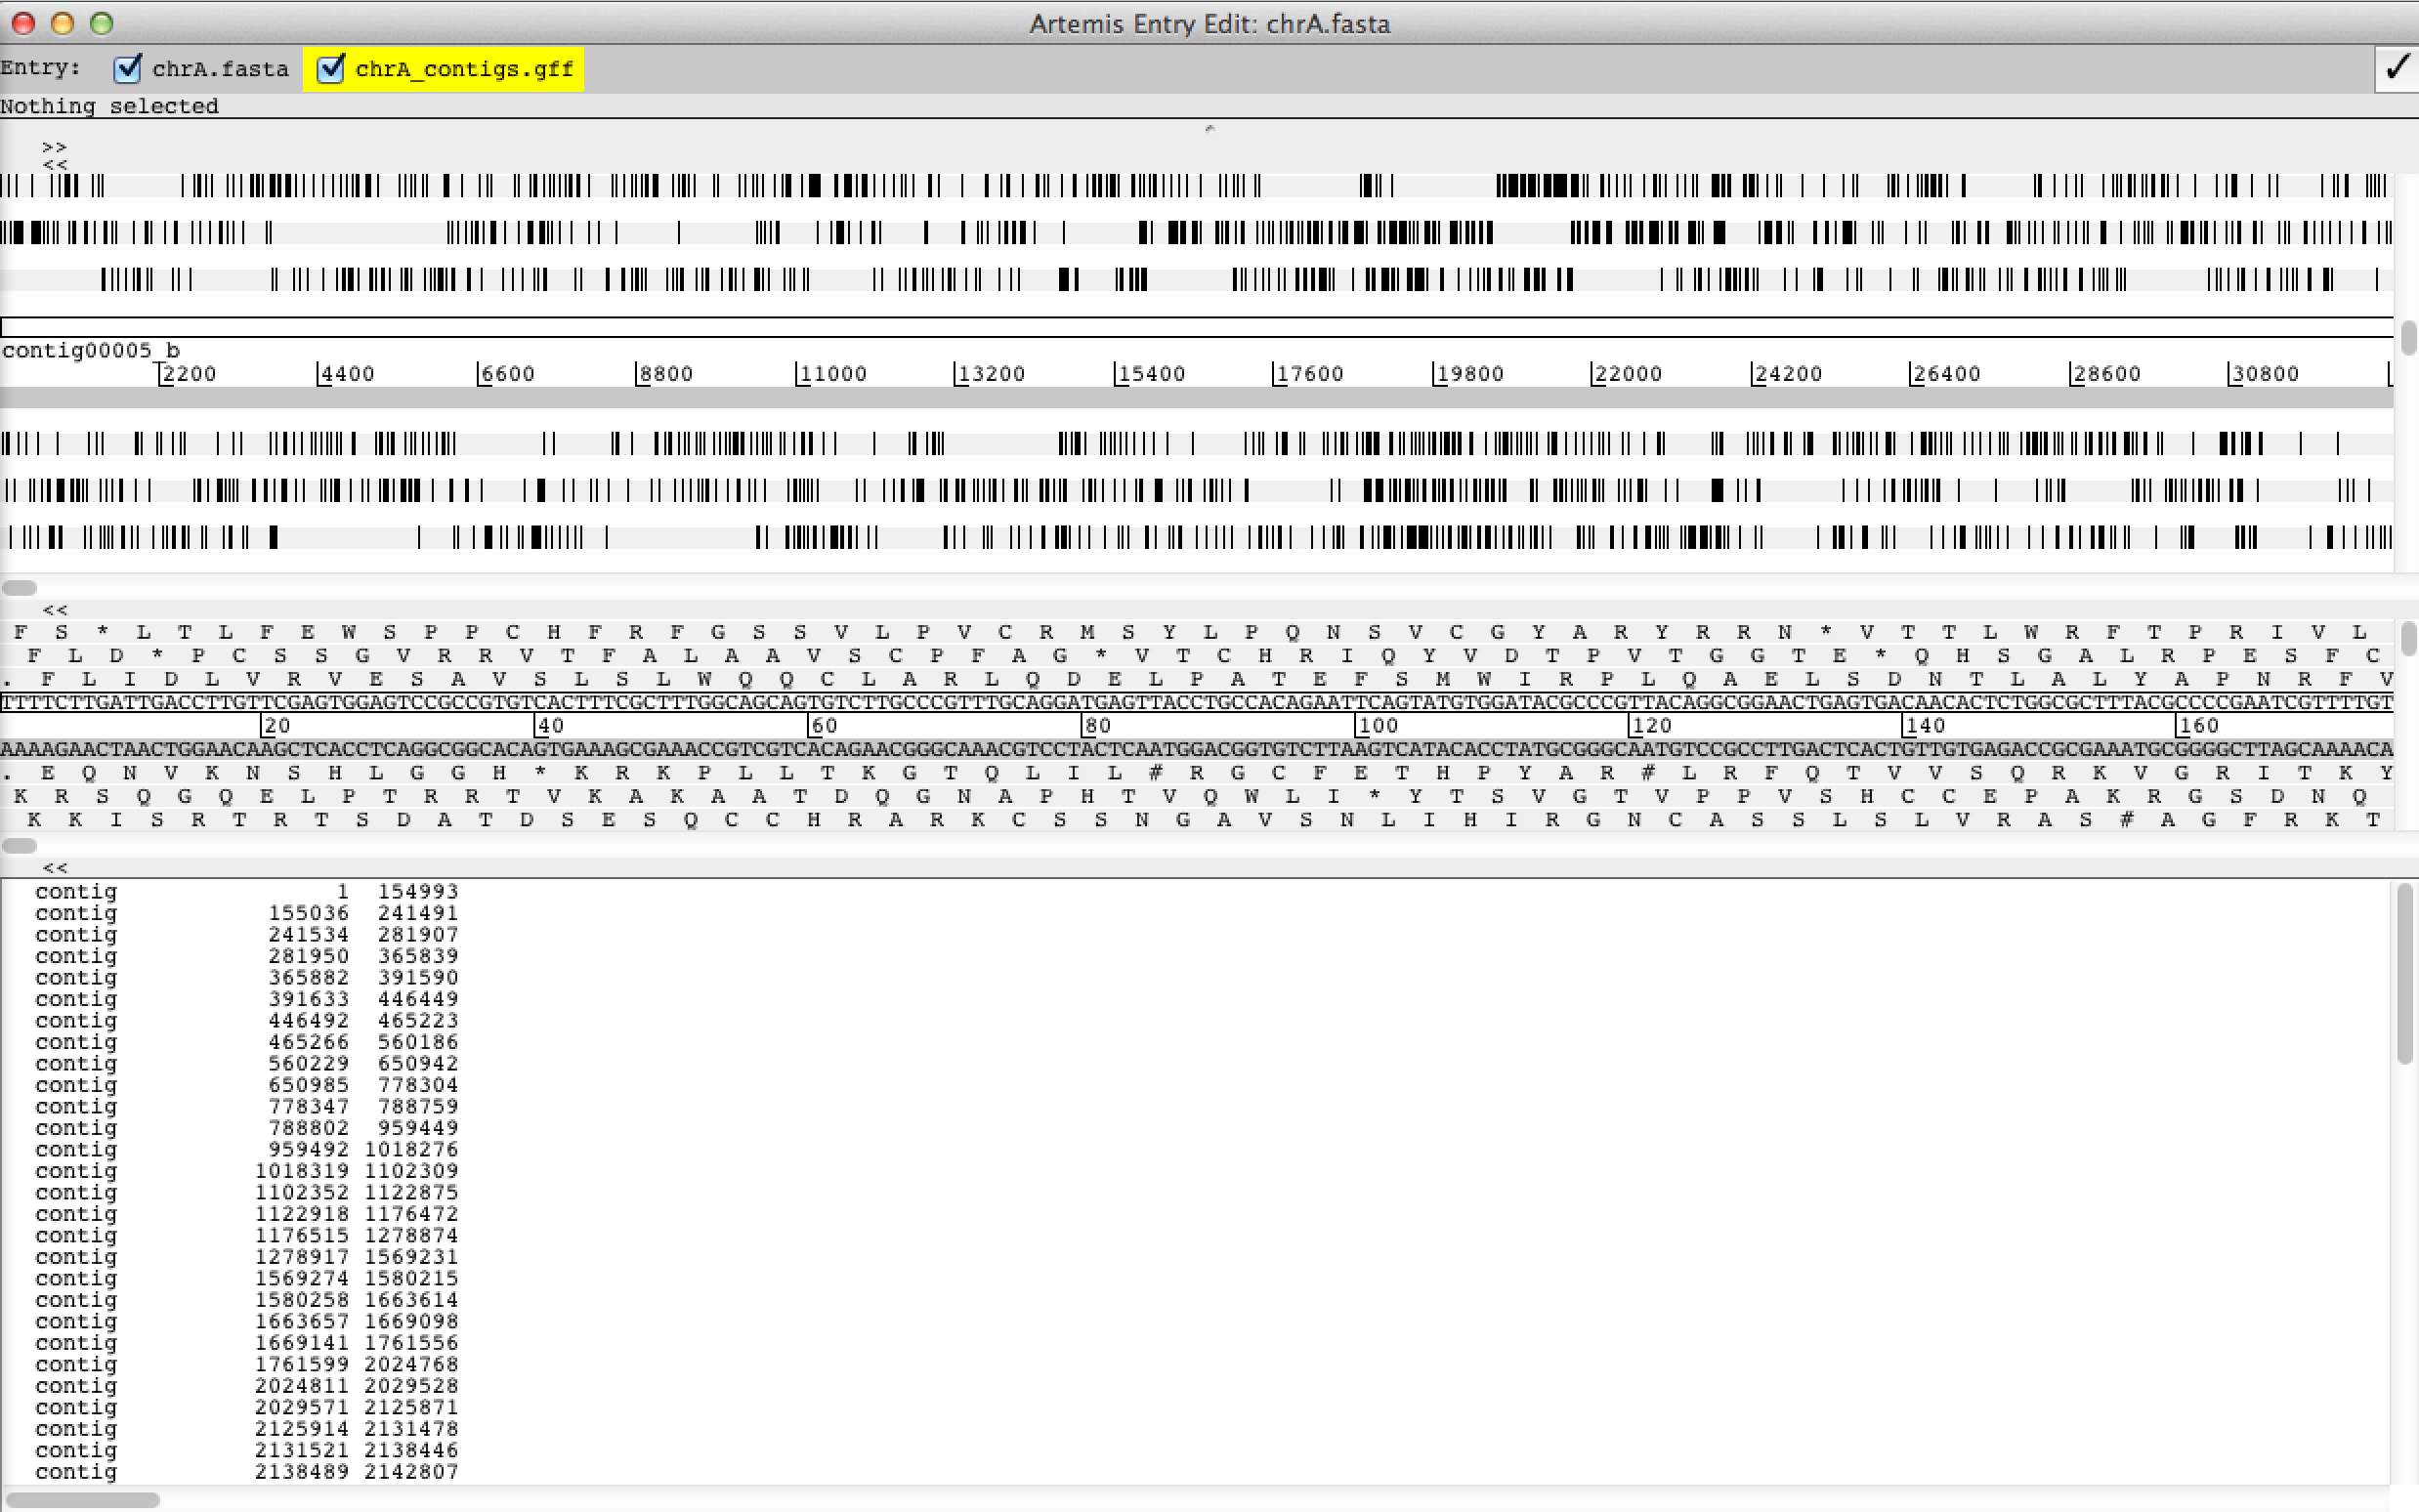
\includegraphics[width=0.9\textwidth]{images/artemis_loaded_contigs} 
    \end{center}
\end{frame}     

  \begin{frame}
    \frametitle{Find the stitching sequence}
    The contigs are stitched with a specific sequence: see if you can find, and identify it.
    \begin{center}
      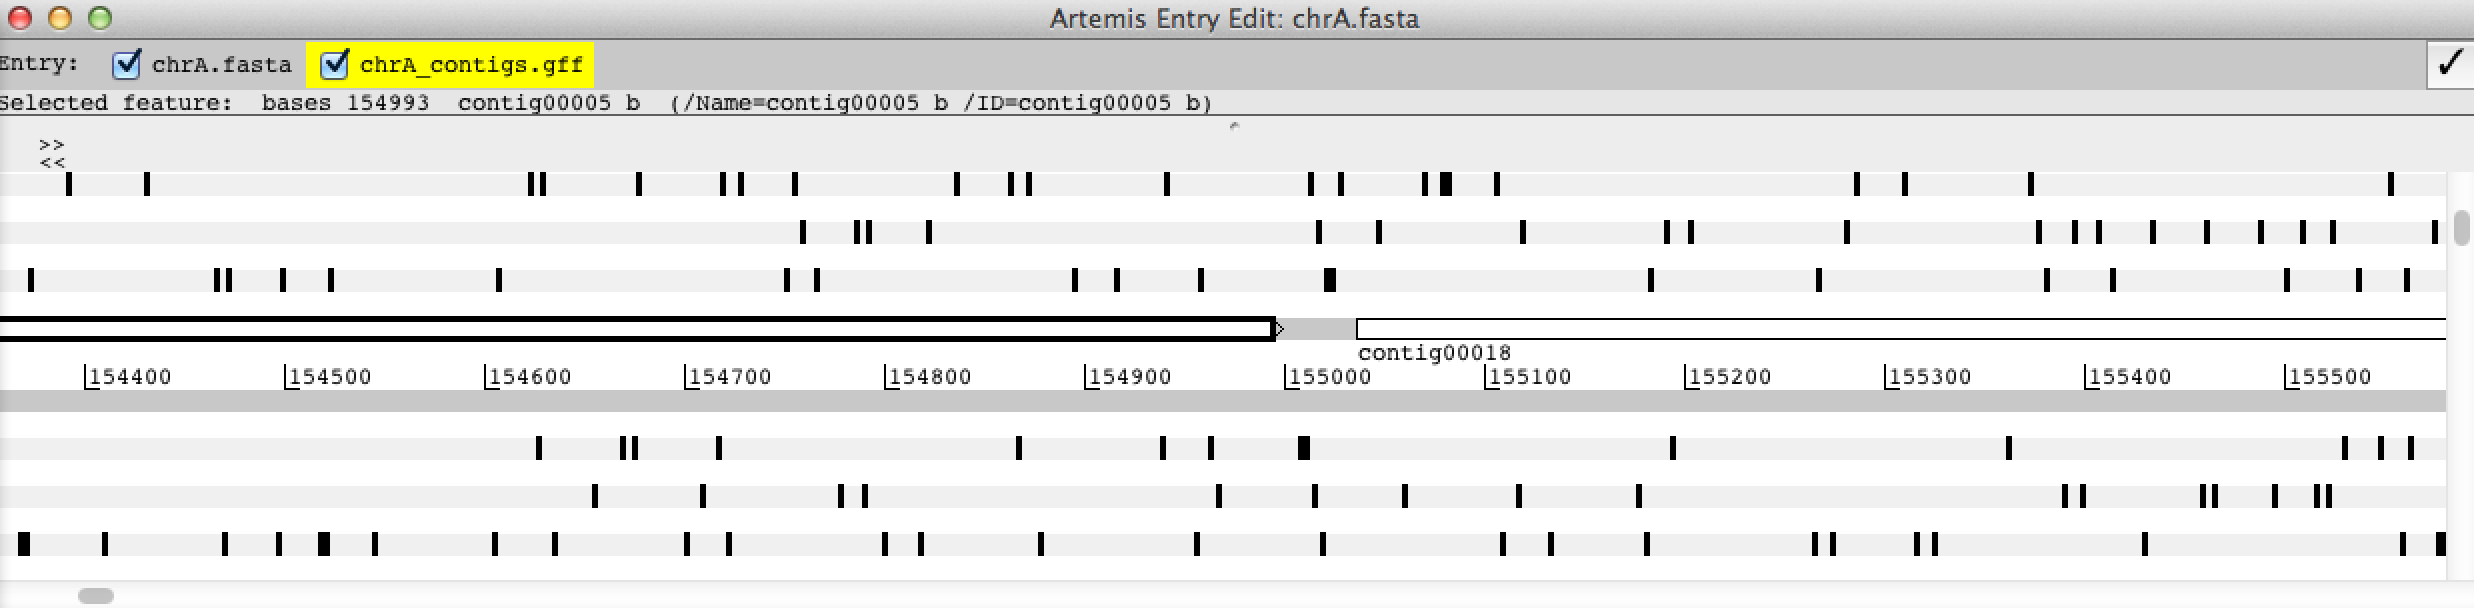
\includegraphics[width=\textwidth]{images/artemis_stitch_tease} 
    \end{center}
\end{frame}     

  % ORF Prediction
  \section{Gene Prediction}
    \begin{frame}
     \frametitle{Methods for gene prediction}
     \begin{itemize}
       \item Homology search
       \item \textit{de novo} prediction
       \begin{itemize}
         \item Unsupervised methods - not trained on a dataset
         \item Supervised methods - trained on a dataset
       \end{itemize}
     \end{itemize}
    \end{frame}  

    \subsection{ORF Prediction}
    \begin{frame}
     \frametitle{ORF Prediction}
     \begin{itemize}
       \item Open Reading Frame = sequence between successive stop codons
       \item A very naive method - unsupervised \textit{de novo} prediction
       \item Sufficiently long ORFs are genes (or exons)
       \item Many tools:
       \begin{itemize}
         \item Artemis
         \item EMBOSS \texttt{getorf}
       \end{itemize}
     \end{itemize}
    \end{frame}  

    \begin{frame}
      \frametitle{ORF Prediction in Artemis}    
      \begin{center}
        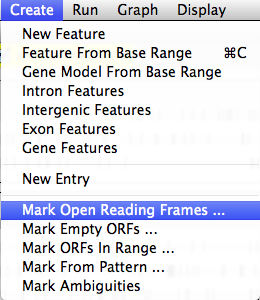
\includegraphics[width=0.3\textwidth]{images/artemis_orf0}     
      \end{center}
    \end{frame} 

    \begin{frame}
      \frametitle{ORF Prediction in Artemis}
      Biological insight required: what size should the smallest ORF be?
      \begin{center}
        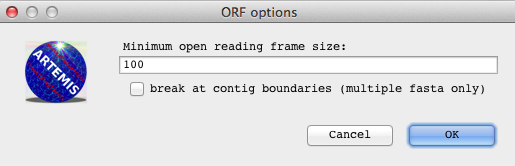
\includegraphics[width=0.9\textwidth]{images/artemis_orf1}     
      \end{center}
    \end{frame} 

    \begin{frame}
      \frametitle{ORF Prediction in Artemis}    
      \begin{center}
        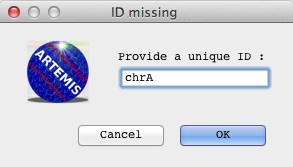
\includegraphics[width=0.9\textwidth]{images/artemis_orf2}     
      \end{center}
    \end{frame} 

    \begin{frame}
      \frametitle{ORF Prediction in Artemis}    
      \begin{center}
        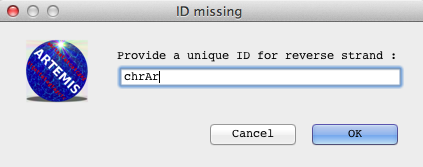
\includegraphics[width=0.9\textwidth]{images/artemis_orf3}     
      \end{center}
    \end{frame} 

    \begin{frame}
      \frametitle{ORF Prediction in Artemis} 
      Is this good enough?
      \begin{center}
        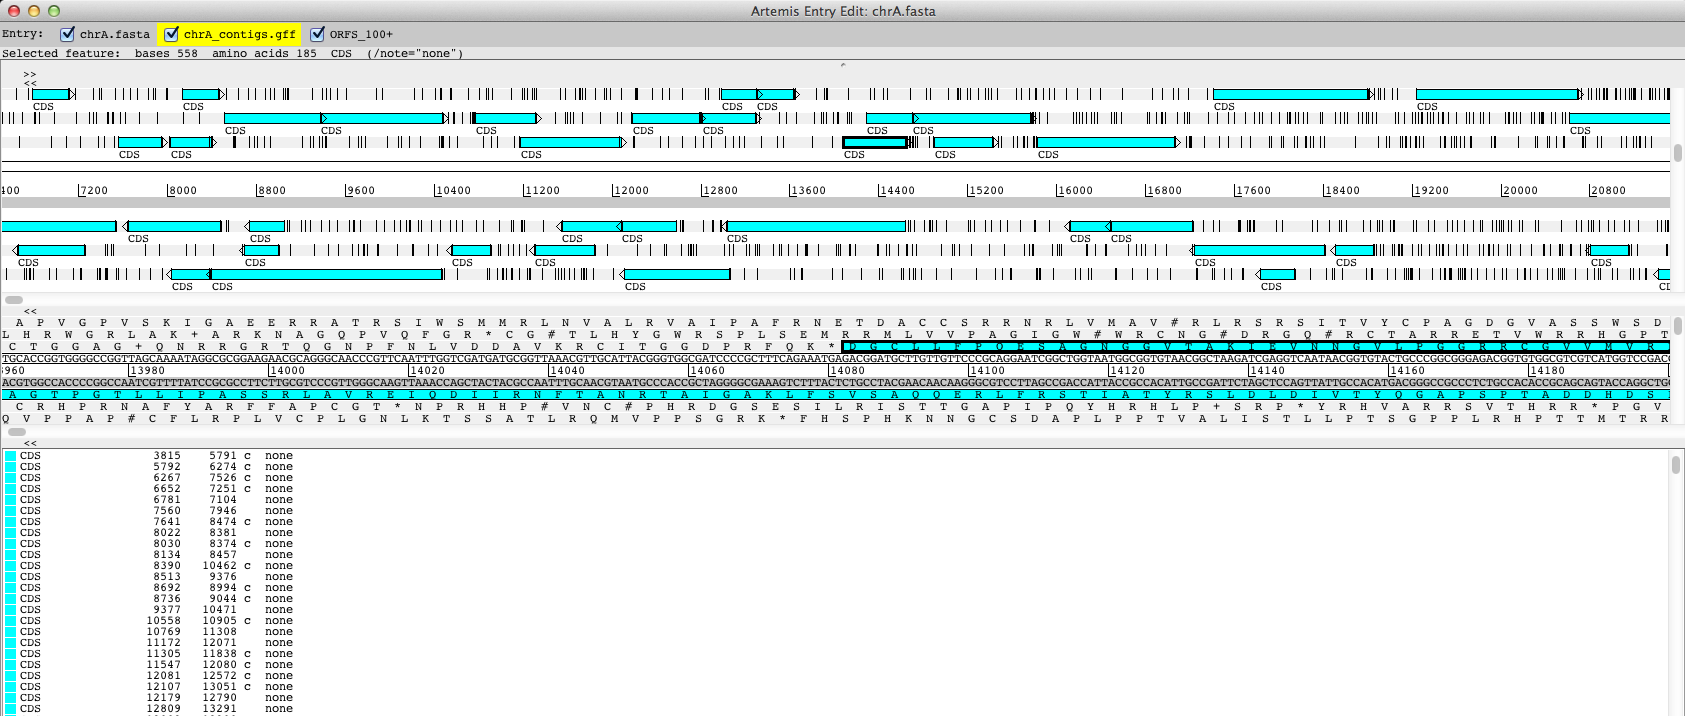
\includegraphics[width=0.9\textwidth]{images/artemis_orf4}     
      \end{center}
    \end{frame} 

    \begin{frame}
      \frametitle{ORF Prediction in Artemis}    
      \begin{center}
        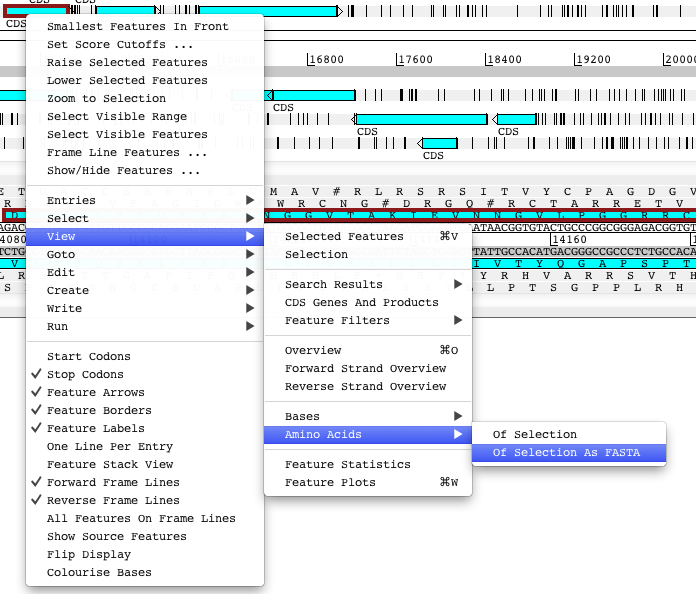
\includegraphics[width=0.7\textwidth]{images/artemis_orf5}     
      \end{center}
    \end{frame} 

    \begin{frame}
      \frametitle{ORF Prediction in Artemis}
      Biological insight: CDS start with start codon.
      \begin{center}
        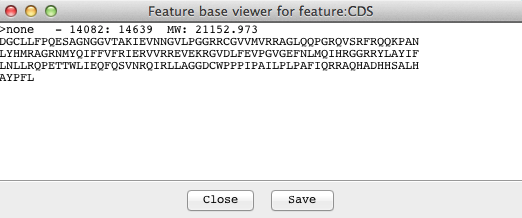
\includegraphics[width=0.9\textwidth]{images/artemis_orf6}     
      \end{center}
    \end{frame} 

    \begin{frame}
      \frametitle{ORF Prediction in Artemis}    
      \begin{center}
        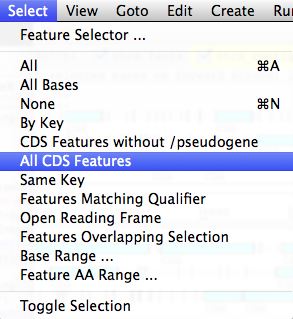
\includegraphics[width=0.5\textwidth]{images/artemis_orf7}     
      \end{center}
    \end{frame} 

    \begin{frame}
      \frametitle{ORF Prediction in Artemis}    
      \begin{center}
        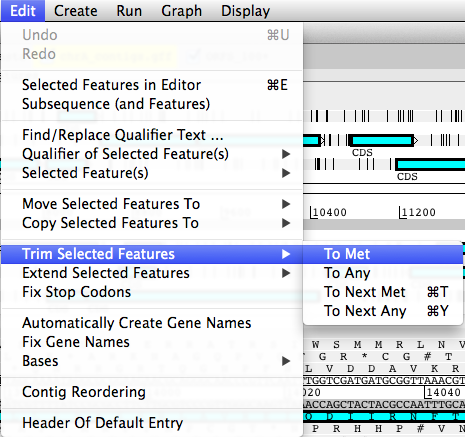
\includegraphics[width=0.6\textwidth]{images/artemis_orf8}     
      \end{center}
    \end{frame} 

    \begin{frame}
      \frametitle{ORF Prediction in Artemis}
      What does this mean, in terms of biology?
      \begin{center}
        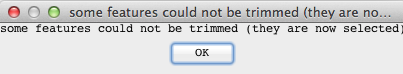
\includegraphics[width=0.9\textwidth]{images/artemis_orf9}     
      \end{center}
    \end{frame} 

    \begin{frame}
      \frametitle{ORF Prediction in Artemis}    
      \begin{center}
        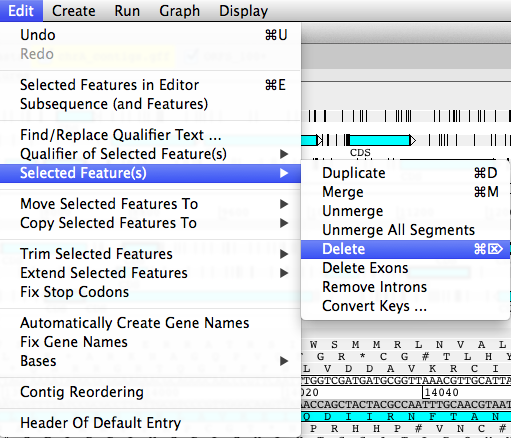
\includegraphics[width=0.6\textwidth]{images/artemis_orf10}     
      \end{center}
    \end{frame} 

    \begin{frame}
      \frametitle{ORF Prediction in Artemis} 
      5410 ORFs with no start codon - how good is ORF detection at finding CDS?
      \begin{center}
        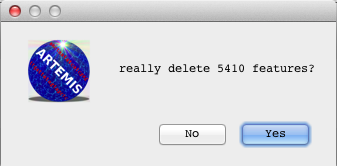
\includegraphics[width=0.9\textwidth]{images/artemis_orf11}     
      \end{center}
    \end{frame} 

    \begin{frame}
      \frametitle{ORF Prediction in Artemis}
      Where do gene names come from?
      \begin{center}
        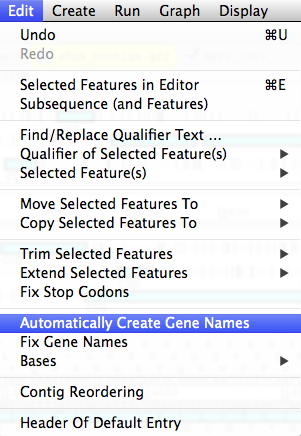
\includegraphics[width=0.3\textwidth]{images/artemis_orf12}     
      \end{center}
    \end{frame} 

    \begin{frame}
      \frametitle{ORF Prediction in Artemis}    
      \begin{center}
        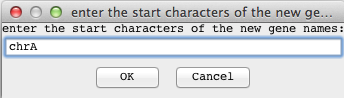
\includegraphics[width=0.9\textwidth]{images/artemis_orf13}     
      \end{center}
    \end{frame} 

    \begin{frame}
      \frametitle{ORF Prediction in Artemis}   
      Is this good enough? 
      \begin{center}
        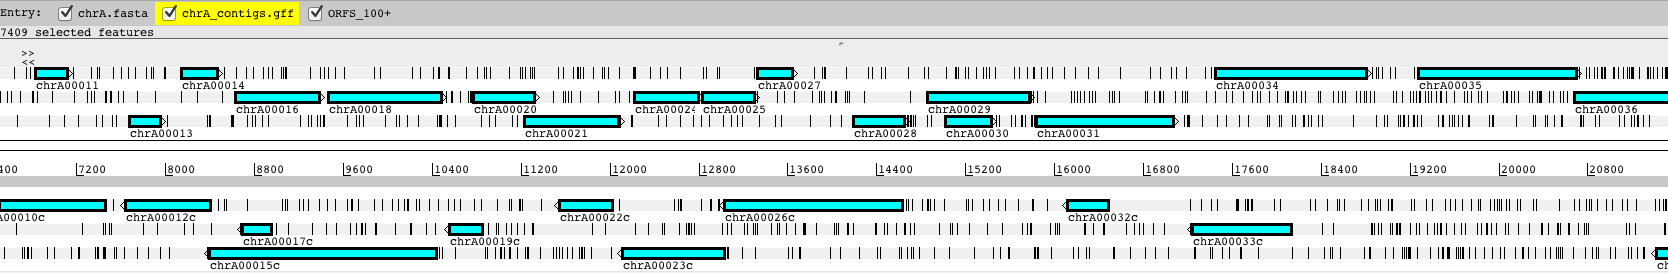
\includegraphics[width=0.9\textwidth]{images/artemis_orf14}     
      \end{center}
      Biological insight: do we expect CDS to overlap like this?
    \end{frame} 

    \begin{frame}
      \frametitle{ORF Prediction in Artemis}   
      \framesubtitle{Lessons learned}   
      \begin{itemize}
        \item ORF finding is very simple
        \item But it still requires biological insight and parameter choices
        \item It's not a very precise way to identify genes or CDS (especially in eukaryotes)
        \item Even in prokaryotes, we only get a candidate set of CDS (many spurious)
      \end{itemize}
    \end{frame} 

    \subsection{CDS Prediction}
    \begin{frame}
     \frametitle{Prokaryotic Prediction Methods}
     \begin{itemize}
       \item Prokaryotes "easier" than eukaryotes for gene prediction
       \begin{itemize}
         \item Very gene-dense (over 90\% of chromosome is coding sequence)
         \item No intron-exon structure
         \item Problem is essentially "which possible ORF contains the true gene, and which start site is correct?"
         \item Still not a solved problem
       \end{itemize}       
     \end{itemize}
    \end{frame}  

    \begin{frame}
     \frametitle{Two Prokaryotic Prediction Methods}
     You will be using two tools
     \begin{itemize}
       \item Glimmer
       \begin{itemize}
         \item Interpolated Markov models
         \item Can be trained on "gold standard" datasets
       \end{itemize}
       \item Prodigal
       \begin{itemize}
         \item Log-likelihood model based on GC frame plots, followed by dynamic programming
         \item Can be trained on "gold standard" datasets
       \end{itemize}
     \end{itemize}
    \end{frame}  

% [fragile] frames must end with \end{frame} directly following a newline, or they break!
  \begin{frame}[fragile]
    \frametitle{Using Glimmer}
    Supervised - we train on a related complete genome sequence, then run \texttt{glimmer3}
    \begin{lstlisting}[language=bash]
$ build-icm -r NC_004547.icm < NC_004547.ffn
$ glimmer3 -o 50 -g 110 -t 30 chrA.fasta NC_004547.icm chrA_glimmer3
    \end{lstlisting}
    \begin{itemize}
      \item \texttt{-o}: max overlap bases
      \item \texttt{-g}: min gene length
      \item \texttt{-t}:  threshold score
    \end{itemize}
\end{frame}  

  \begin{frame}[fragile]
    \frametitle{Using Glimmer}
    \texttt{glimmer3} output is non-standard
    \begin{lstlisting}[language=bash]
$ head -n 4 chrA_glimmer3.predict 
>chrA
orf00001       36     1430  +3     8.81
orf00002     1435     2535  +1    11.51
orf00005     2676     3761  +3     8.63
    \end{lstlisting}
    We could Google for help, or just hack together a short script
    \begin{lstlisting}[language=bash]
$ python glimmer_to_gff.py chrA_glimmer3.predict
    \end{lstlisting}    
\end{frame}  

  \begin{frame}[fragile]
    \frametitle{Using Glimmer}
    We now have output in GFF
    \begin{lstlisting}[language=bash]
$ head -n 3 chrA_glimmer3.gff 
chrA	Glimmer	CDS	36	1430	8.81	+	0	ID=orf00001;Name=orf00001
chrA	Glimmer	CDS	1435	2535	11.51	+	0	ID=orf00002;Name=orf00002
chrA	Glimmer	CDS	2676	3761	8.63	+	0	ID=orf00005;Name=orf00005
    \end{lstlisting}
\end{frame}  

% [fragile] frames must end with \end{frame} directly following a newline, or they break!
  \begin{frame}[fragile]
    \frametitle{Using Prodigal}
    Unsupervised (i.e. untrained) mode
    \begin{lstlisting}[language=bash]
$ prodigal -f gff -o chrA_prodigal.gff -i chrA.fasta
    \end{lstlisting}
\end{frame}  

% [fragile] frames must end with \end{frame} directly following a newline, or they break!
  \begin{frame}[fragile]
    \frametitle{Using Prodigal}
    Prodigal GFF output is correctly formatted and informative
    \begin{lstlisting}[language=bash]
$ head -n 6 chrA_prodigal.gff 
##gff-version  3
# Sequence Data: seqnum=1;seqlen=4727782;seqhdr="chrA"
# Model Data: version=Prodigal.v2.50;run_type=Single;model="Ab initio";gc_cont=54.48;transl_table=11;uses_sd=1
chrA	Prodigal_v2.50	CDS	3	1430	188.5	+	0	ID=1_1;partial=10;start_type=Edge;rbs_motif=None;rbs_spacer=None;score=188.54;cscore=185.37;sscore=3.18;rscore=0.00;uscore=3.18;tscore=0.00
chrA	Prodigal_v2.50	CDS	1435	2535	185.6	+	0	ID=1_2;partial=00;start_type=ATG;rbs_motif=None;rbs_spacer=None;score=185.61;cscore=184.24;sscore=1.36;rscore=-7.73;uscore=3.48;tscore=4.37
chrA	Prodigal_v2.50	CDS	2676	3761	146.2	+	0	ID=1_3;partial=00;start_type=ATG;rbs_motif=None;rbs_spacer=None;score=146.19;cscore=149.82;sscore=-3.63;rscore=-7.73;uscore=-0.28;tscore=4.37
    \end{lstlisting}
\end{frame}  

    \begin{frame}
     \frametitle{Comparing predictions in Artemis}
      \begin{center}
        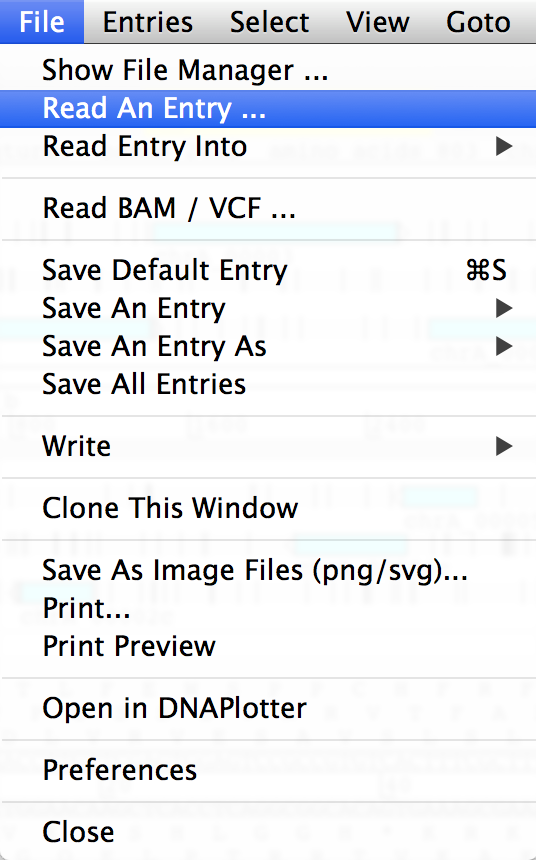
\includegraphics[width=0.3\textwidth]{images/artemis_cdspred0}     
      \end{center}
    \end{frame}  

    \begin{frame}
     \frametitle{Comparing predictions in Artemis}
      \begin{center}
        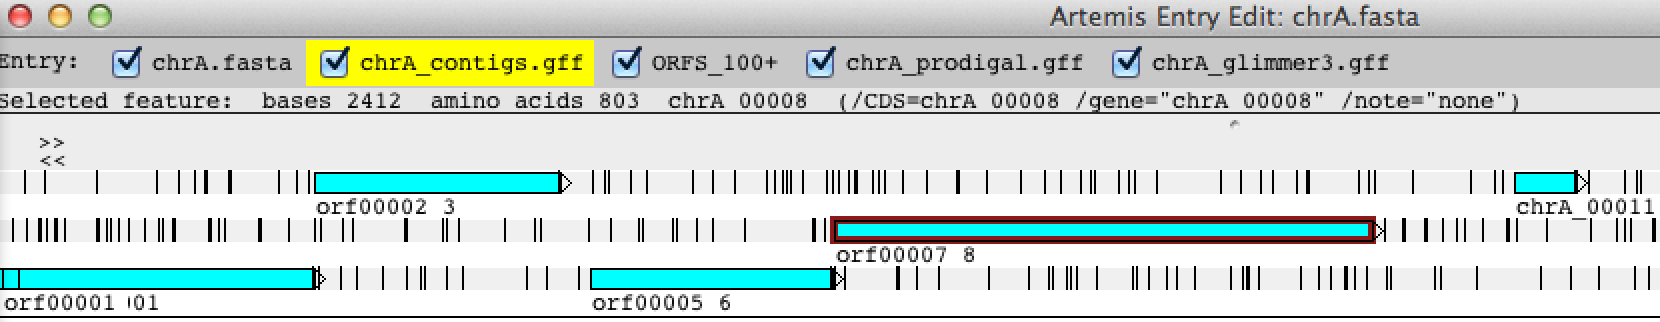
\includegraphics[width=0.9\textwidth]{images/artemis_cdspred1}     
      \end{center}
    \end{frame}  

    \begin{frame}
     \frametitle{Comparing predictions in Artemis}
      \begin{center}
        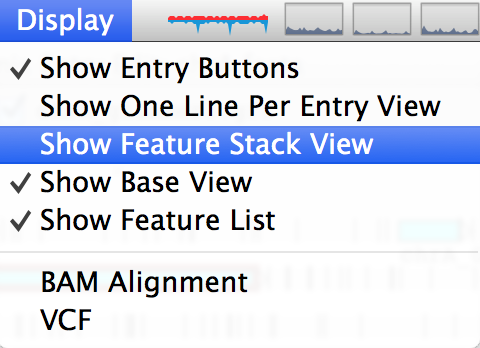
\includegraphics[width=0.4\textwidth]{images/artemis_cdspred2}     
      \end{center}
    \end{frame}  

    \begin{frame}
     \frametitle{Comparing predictions in Artemis}
     Do ORF(orange)/CDS(green,blue) prediction methods agree?
      \begin{center}
        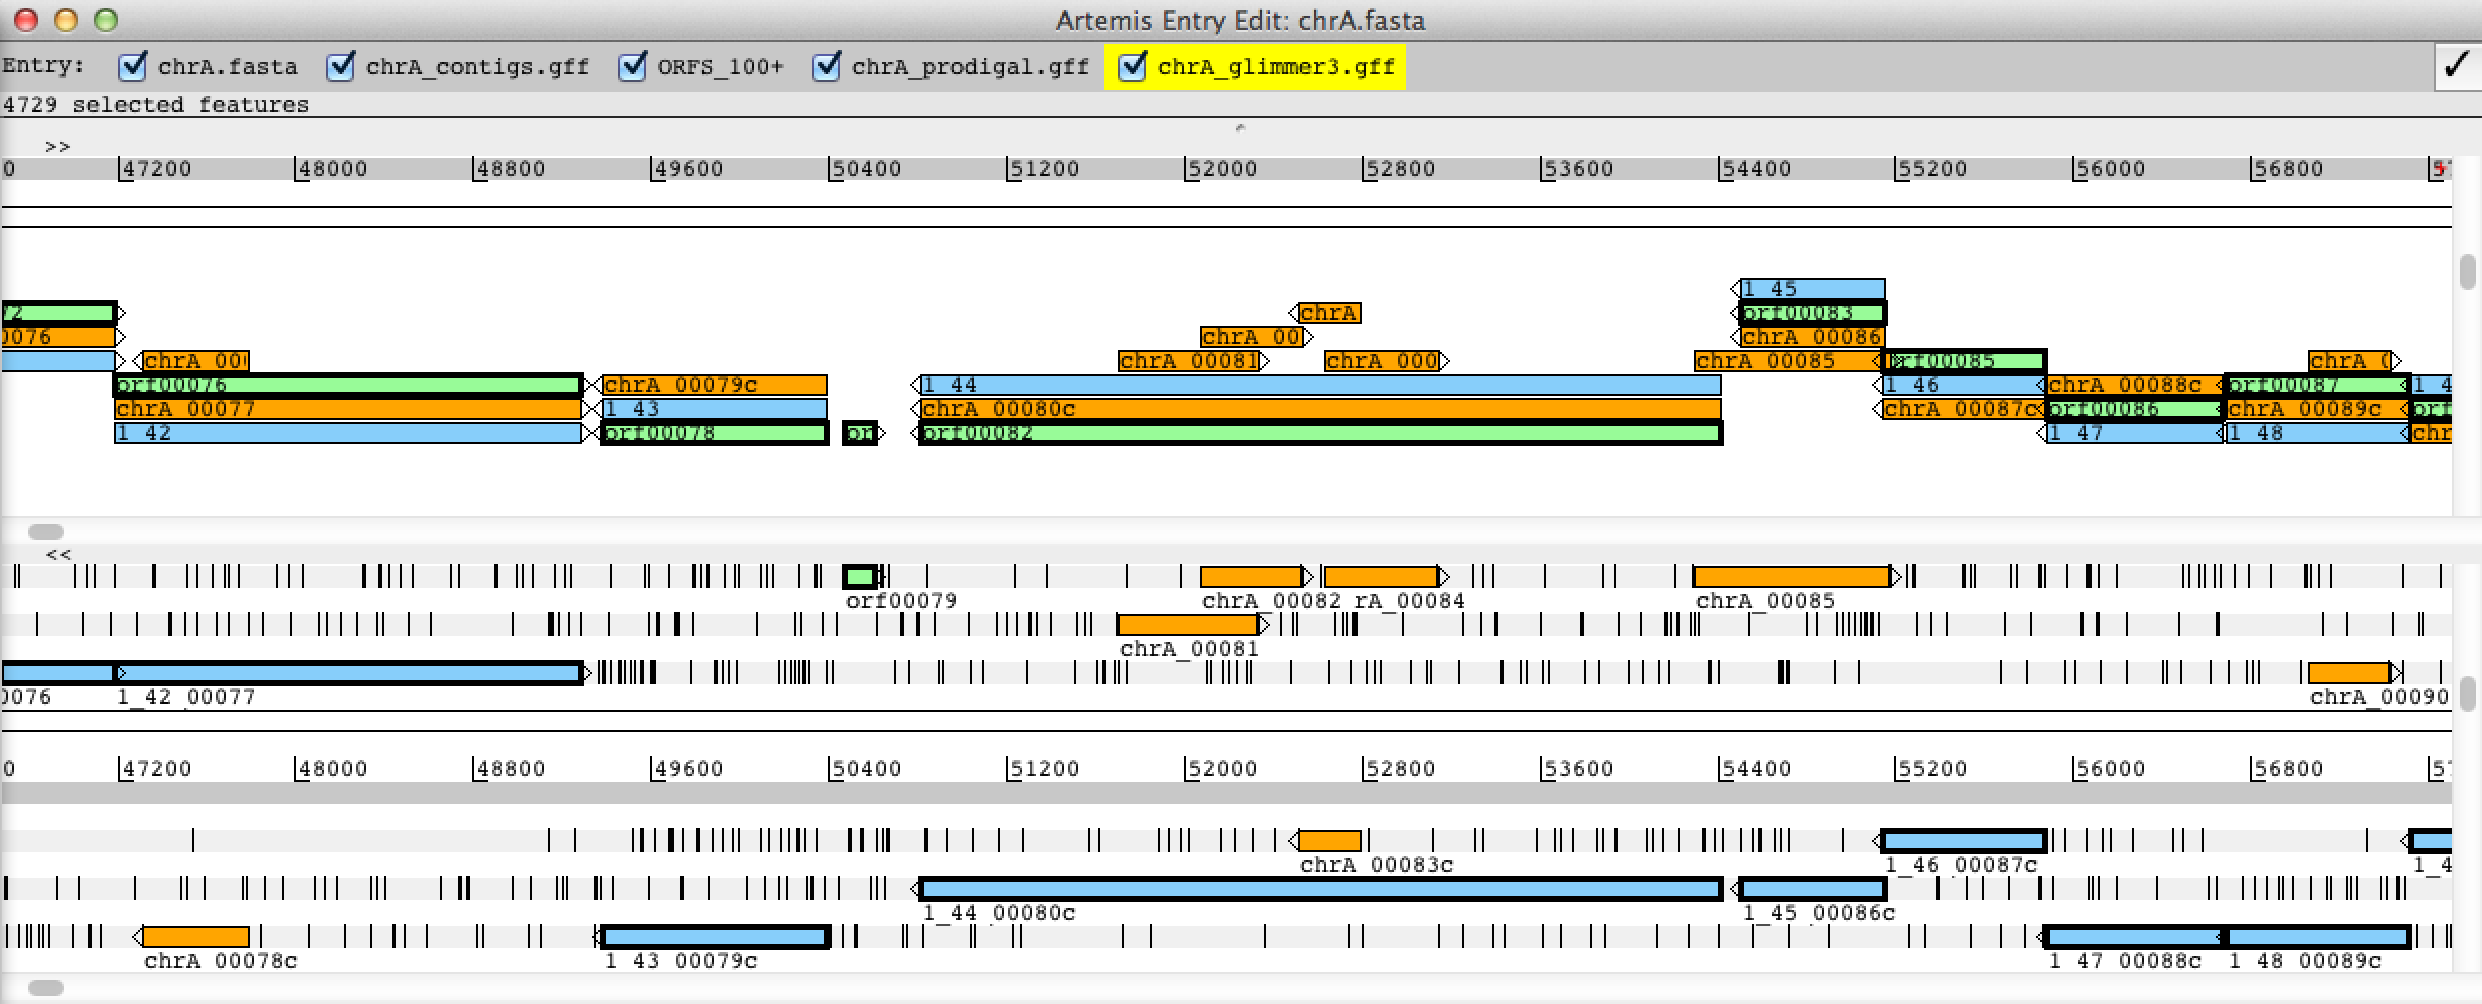
\includegraphics[width=0.9\textwidth]{images/artemis_cdspred3}     
      \end{center}
    \end{frame}  

    \begin{frame}
     \frametitle{Comparing predictions in Artemis}
     Do \texttt{glimmer}(green)/\texttt{prodigal}(blue) CDS prediction methods agree?
      \begin{center}
        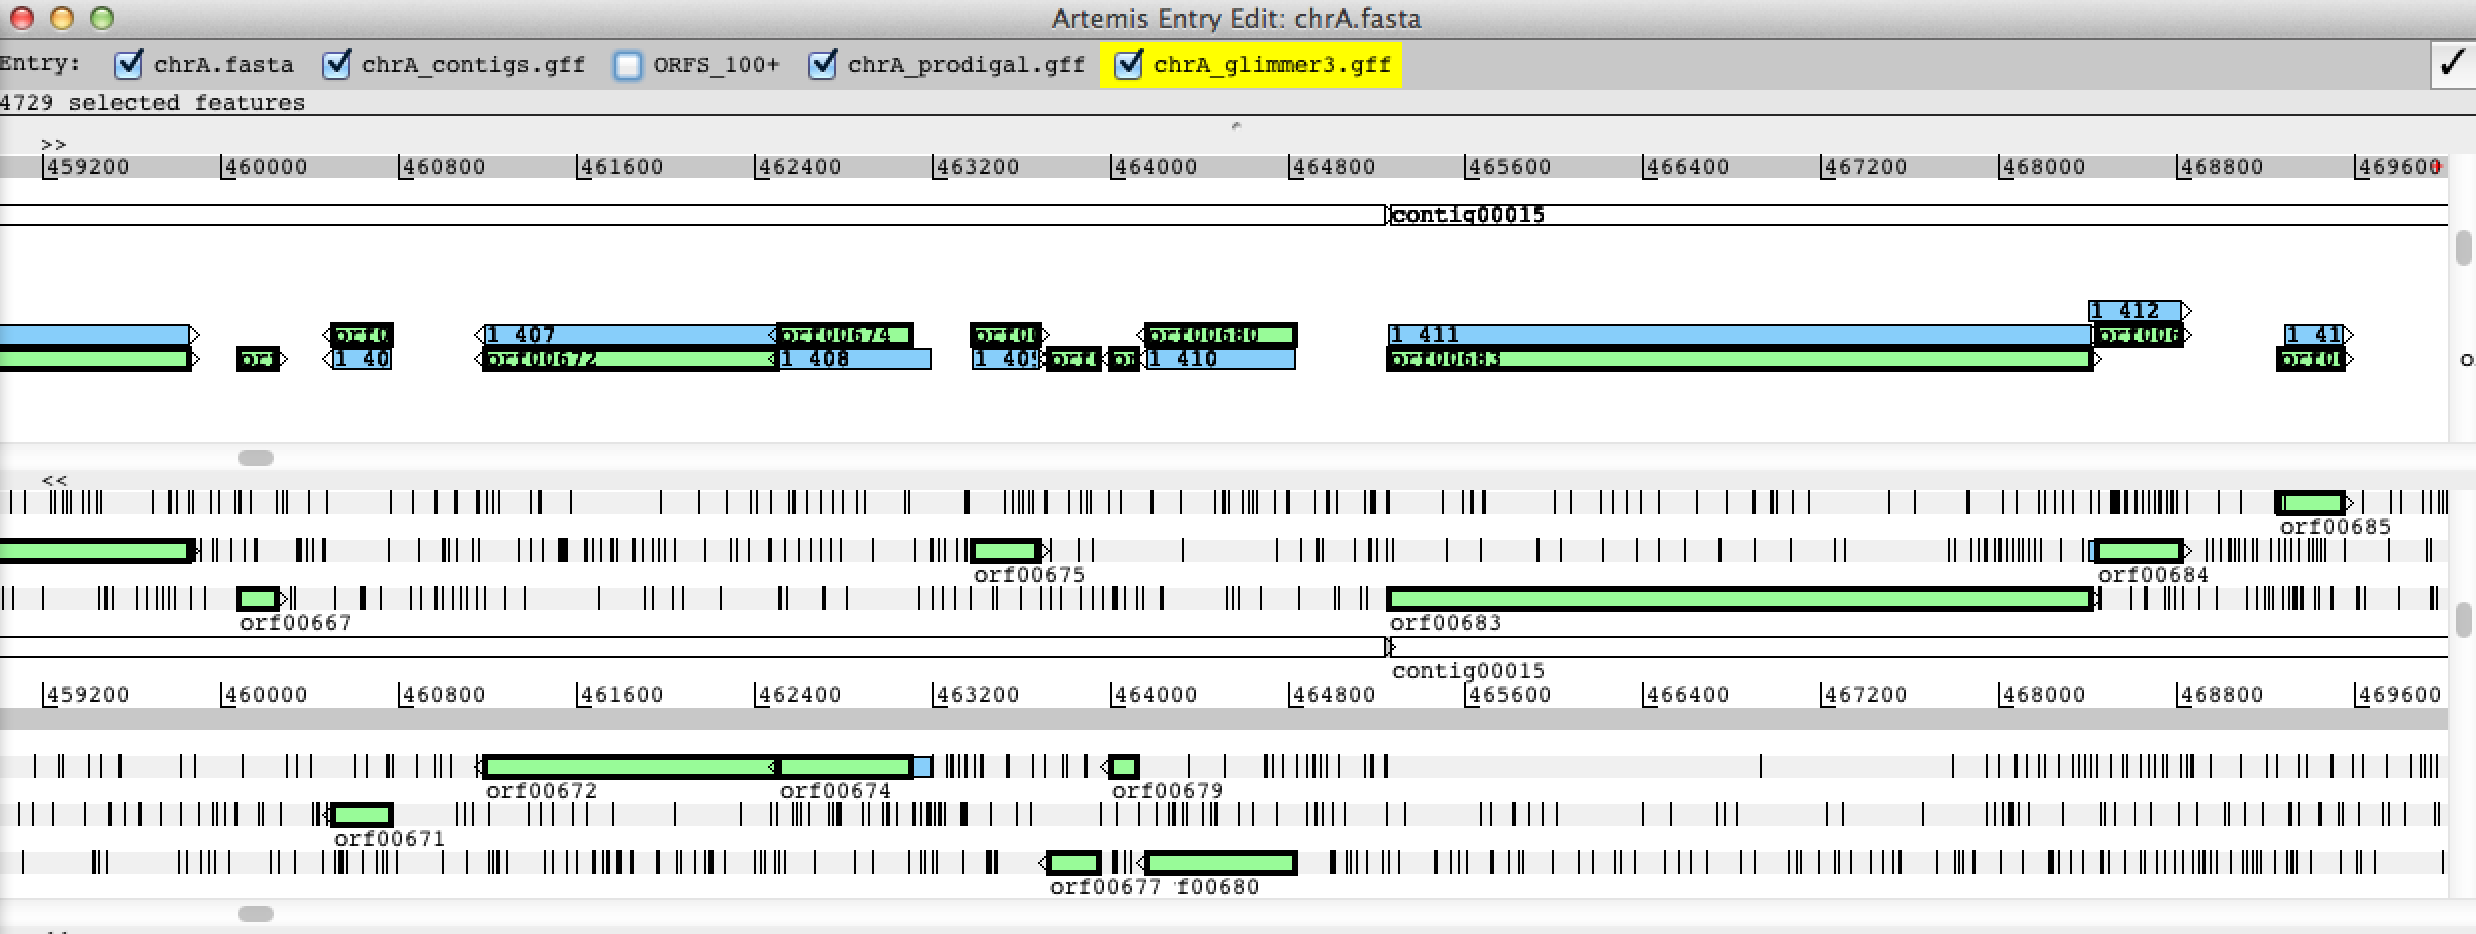
\includegraphics[width=0.9\textwidth]{images/artemis_cdspred4}     
      \end{center}
      How do we know which is best?
    \end{frame}  

    \subsection{Assessing Prediction Methods}
    \begin{frame}
     \frametitle{Using a "Gold Standard"}
     \begin{itemize}
       \item 
     \end{itemize}
    \end{frame} 


  % BLAST comparisons
  \section{Genome comparisons}
% [fragile] frames must end with \end{frame} directly following a newline, or they break!
  \begin{frame}[fragile]
    \frametitle{Run a megaBLAST Comparison}
    Make a new working directory, and BLAST your chromosome against the comparator sequence \\
    Put results in \texttt{chrA\_megablast\_Pba.tab}
    \begin{lstlisting}[language=bash]
$ pwd
[...]/Introduction_To_Bioinformatics
$ mkdir workshop
$ cd workshop
$ blastn -query ../data/workshop/chromosomes/chrA.fasta -subject ../data/workshop/chromosomes/NC_004547.ffn -out chrA_megablast_Pba.tab -outfmt 6 
$ head -n 3 chrA_megablast_Pba.tab 
chrA	gi|50118965|ref|NC_004547.2|:10948-12453	80.34	1511	287	10	4579450	4580955	1506	1	0.0	1136
chrA	gi|50118965|ref|NC_004547.2|:c33859-32447	82.04	1409	253	0	4563151	4564559	1	1409	0.0	1201
chrA	gi|50118965|ref|NC_004547.2|:c34917-33868	82.48	1050	184	0	4562093	4563142	1	1050	0.0	 920
    \end{lstlisting}
\end{frame} 
    
% [fragile] frames must end with \end{frame} directly following a newline, or they break!
  \begin{frame}[fragile]
    \frametitle{Run a BLASTN Comparison}
    Make a new working directory, and BLAST your chromosome against the comparator sequence \\
    Put results in \texttt{chrA\_blastn\_Pba.tab}
    \begin{lstlisting}[language=bash]
$ pwd
[...]/Introduction_To_Bioinformatics
$ mkdir workshop
$ cd workshop
$ blastn -query ../data/workshop/chromosomes/chrA.fasta -subject ../data/workshop/chromosomes/NC_004547.ffn -out chrA_blastn_Pba.tab -outfmt 6 -task blastn
$ head -n 3 chrA_blastn_Pba.tab 
chrA	gi|50118965|ref|NC_004547.2|:5629-7497	79.68	1865	379	0	4584915	4586779	1865	1	0.0	1654
chrA	gi|50118965|ref|NC_004547.2|:5629-7497	92.59	27	2	0	4479367	4479393	1254	1280	0.004	41.0
chrA	gi|50118965|ref|NC_004547.2|:5629-7497	100.00	17	0	0	4613022	4613038	52	36	2.1	31.9
    \end{lstlisting}
\end{frame}     
    
% [fragile] frames must end with \end{frame} directly following a newline, or they break!
  \begin{frame}[fragile]
    \frametitle{Do BLASTN and megaBLAST comparisons agree?}
    Check the number of alignments returned with \texttt{wc}
    \begin{lstlisting}[language=bash]
$ wc chrA_megablast_Pba.tab 
     536    6432   52969 chrA_megablast_Pba.tab
$ wc chrA_blastn_Pba.tab 
    4425   53100  429478 chrA_blastn_Pba.tab
    \end{lstlisting}
    What is this telling us? \\
    Why do the results differ?
\end{frame}         

  \begin{frame}
    \frametitle{BLASTN vs megaBLAST}
    \begin{itemize}
      \item<1-> BLASTN uses the BLAST algorithm, megaBLAST does not
      \begin{itemize}
        \item (though BLAST+ BLASTN now uses megaBLAST by default)
      \end{itemize}      
      \item<1-> megaBLAST uses a fast, greedy algorithm due to Zhang et al. (2000) \url{http://www.ncbi.nlm.nih.gov/pubmed/10890397}
      \item<2-> megaBLAST is optimised for
      \begin{itemize}
        \item genome-level searches
        \item queries on large sequence sets (automatic query packing)
        \item long alignments of similar sequences, with SNPs/sequencing errors
      \end{itemize}
      \item<2-> A discontinuous mode (dc-megaBLAST) is recommended for more divergent sequences
    \end{itemize}
\end{frame}   
    
% etc
\end{document}